\chapter{Background}
  \section{Previous Work}
    \subsection{Defining the Internet of Things}
      The Internet of Things is a high-level concept which encompasses many ideas and technologies, and this makes it difficult to define absolutely. In this respect it is similar to Cloud Computing. Cloud Computing has come to represent different forms to different stakeholders, whether they are application developers, infrastructure engineers or end users. As the concept matured through research, conferences and industrial uptake, Cloud Computing has become identified by its use-cases and marketing jargon. For instance the industry has come to recognise Infrastructure-as-a-Service (IaaS), Platform-as-a-Service (PaaS) or Software-as-a-Service (SaaS) as characteristics of the Cloud Computing concept \citep{viewOfCloud}. History may repeat itself with the Internet of Things where the definition will be refined as uptake and research improves.

      In the mean time we can begin plotting the footprint of IoT. The term `Internet of Things' captures the essence of the vision well; the vision of a world where everyday, physical objects are gateways to web-based services. These so-called `smart objects' comprise of sensors to perceive their environment or context, as well as a notion of inter-connectivity with other objects or services. Connected objects or services may react to collected data to trigger actions, and these actions may be digital or physical. The Internet of Things could be summarised as data collection, aggregation and reaction in the physical domain.

      The boundaries between IoT and other trends help to define its place in computing. For instance the research area of Wireless Sensor Networks (WSN) carries similarities in hardware requirements and challenges. In particular, WSN comprise of connected sensors and actuators \citep{Mottola:2011}. This differs from IoT because of the scope of connectivity; the closed-loop fashion of WSNs limit their potential to specific use-cases whereas the global context of IoT allows for a wider range of applications. Wireless Sensor Networks can form one layer of an Internet of Things application.

      The research area of `Wearables' also overlaps with the Internet of Things. Wearables are `smart' devices designed to be worn or embedded within the body and combine sensors and some form of connectivity, typically integrating with a smartphone \citep{6844949, evrything}. Consumer Wearables products are already on the shelves, such as Fitbit---a wrist-worn personal health tracker. The Fitbit wristband connects to a smartphone with Bluetooth Low Energy (BLE) and this smartphone then provides global connectivity through its wireless connection. Users can sign-in to a web-based dashboard which will collate and organise personal data. In this scenario, Wearables are collecting, aggregating and reacting to data in the physical domain. Wearables could therefore be described as a subset of the Internet of Things---they are an application in a specific domain.

      Two trends which acknowledge the vastness of information technology are `Ubiquitous Computing' and `Big Data'. The Ubiquitous Computing concept describes an environment where users are surrounded by connected technology---technology in our homes, workplaces and recreational activities. \cite{Weiser:1999} notes that ``specialized elements of hardware and software, connected by wires, radio waves and infrared, will be so ubiquitous that no one will notice their presence'' and this is reflective of the vision for Internet of Things. If Ubiquitous Computing describes a physical world saturated with sensors and devices then Big Data describes a \emph{digital} world saturated with huge datasets. These datasets will have different origins and so their structures may differ too; it is the purpose of Big Data to normalise and analyse these on a massive scale. The Internet of Things could be seen as a specific use case for both Ubiquitous Computing and Big Data.

      As we have seen, the boundary of the Internet of Things overlaps with other trends in computing. Figure \ref{iotRelationship} exemplifies the extent of which the definition of IoT relies on these related fields. What can be taken away about the definition of the Internet of Things is that it focuses on not just one idea or technology but rather a collection of them.

      \begin{figure}
        \centering
          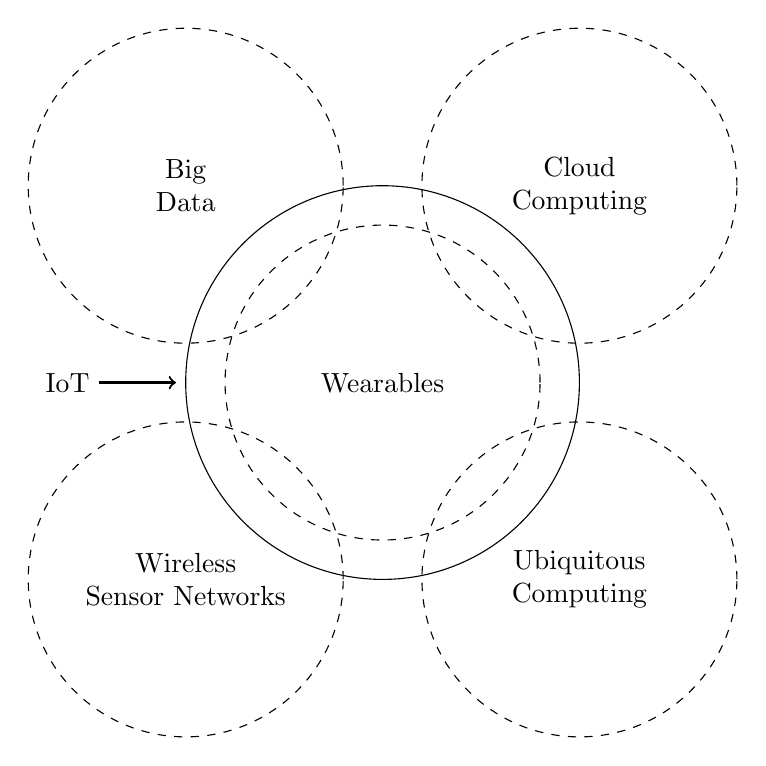
\begin{tikzpicture}
            \node (IoT) at (-2.5,0) {};
            \node at (-4,0) {IoT} edge[->,thick,out=0,in=180] (IoT);
            \draw (0,0) circle [radius=2.5];

            \node[align=center] at (0,0) {Wearables};
            \draw [dashed] (0,0) circle [radius=2];

            \node[align=center] at (-2.5,2.5) {Big\\Data};
            \draw [dashed] (-2.5,2.5) circle [radius=2];

            \node[align=center] at (2.5,2.5) {Cloud\\Computing};
            \draw [dashed] (2.5,2.5) circle [radius=2];

            \node[align=center] at (-2.5,-2.5) {Wireless\\Sensor Networks};
            \draw [dashed] (-2.5,-2.5) circle [radius=2];

            \node[align=center] at (2.5,-2.5) {Ubiquitous\\Computing};
            \draw [dashed] (2.5,-2.5) circle [radius=2];
          \end{tikzpicture}
        \caption{Describing the Internet of Things with other trends in computing}\label{iotRelationship}
      \end{figure}

    \subsection{Opportunities}
      Why should we develop Internet of Things solutions? Would our society actually benefit from them? These are the questions posed by businesses, consumers, software developers and academics alike. Pilot projects as well as industrial and academic research have shown that there are wide-reaching opportunities to be grasped. Until recently, these opportunities were achievable only in theoretical, lab-based scenarios but due to the advancements in the supporting technology, they are more achievable for real-world industries.

      The technical capabilities of hardware, the readiness of software and all of their associated costs are prominent blockers to the IoT industry. Advancements in the hardware---smaller, more powerful and more efficient microcontrollers---mean that smart objects are technologically more feasible. Large industry players, such as Intel and Samsung, have brought to market the their own IoT hardware platforms---Intel's Edison System on a Chip (SoC) and Samsung's Artik family of boards. Improvements in the mass production of these also reduce financial barriers, making investment more feasible for businesses. The real-world opportunities presented before us can be categorised into two main areas: economic \& societal and technical.

      \subsubsection{Economic and Societal}
        Irrespective of the industry or domain, the ultimate purpose of Internet of Things is to help people. From the perspective of a service, these applications do and should provide value on an individual basis, however the real value is found with the network effect of interconnected products and services. Both the Internet of Things and societies of people are similar in that their wholes are greater than the sum of their parts.

        The European Union (EU) is a prime example of a society which can benefit from the Internet of Things. It is special because it represents the needs and wants of not just one nation but a collection of nations. The European Commission is the governmental body of the EU, which itself recognises the potential in IoT: ``One major next step in this development [of the Internet] is to progressively evolve from a network of interconnected computers to a network of interconnected objects, from books to cars, from electrical appliances to food, and thus create an ‘Internet of things’.'' In 2009 the Commission published an action plan for embracing the Internet of Things.

        The action plan notes two main areas of opportunity: citizen well-being and economic prosperity. The improved well-being of citizens is achieved through specific and targeted use-cases. For instance internet-connected health monitoring systems could alleviate pressure on medical services for the ageing society, or smart waste management with products which can describe their contents would help to reduce their carbon footprint. The improvement of economic prosperity is achieved through organised and systematic uptake of the Internet of Things. By leading the development of IoT rather than accepting the standards of other nations, the EU can drive development for the benefit of its own industries.

        Although there are strong opportunities for individuals and political territories, the best economic opportunites are available to businesses. The Internet of Things has the potential to provide many new income streams to businesses as well as finding other money through efficiency savings. First of all IoT opens up new markets which were previously not feasible nor even considered. These markets may include consumer products such as the previously mentioned Fitbit or novel service solutions such as home security and monitoring. For organisations with complex supply chains or processes, the Internet of Things could help to maximise resources and stock control. This is especially evident in areas such as logistics or public transport where connected devices could help to reduce costs by optimising transportation routes automatically.

      \subsubsection{Technical}
        Technical opportunities and advancements are self-perpetuating and really are the driving force behind the Internet of Things. As previously noted, IoT would not be realistically possible without improvements in the underlying technology. As more powerful, efficient and cheaper hardware boards are delivered and as they become supported by software layers, the possible use-cases of them diversifies too.

        \citet{fromIoC} note that the Internet of Things is not the result of a single novel technology but rather several complementary technical developments. These technical developments provide a range of capabilities, or in the eyes of an application stakeholder, technical \emph{opportunities}. The main opportunities presented are: communication and cooperation; addressability; identification; sensing; actuation; localisation; embedded information processing and user interfaces. The authors also note that most applications will need only a subset of these capabilities, but it is better to have the option there.

        The value of the Internet of Things is derived from the communication of data---either human-to-machine, machine-to-human or machine-to-machine. This trait makes the capabilities of communication and cooperation, addressability and identification particularly important to its success. Objects with the ability to network between themselves or other Internet services are clearly key. While the Internet will provide the backbone for this, it is the Wireless Personal Area Network technologies which present the opportunities---technologies such as GSM, Wi-Fi, Bluetooth, ZigBee and 6LoWPAN. These technologies in conjunction with other technology layers allow devices to be uniquely identified and addressed from anywhere in the world. With this global interconnectivity, the possibilities really do open up.

        The second main characteristic of IoT is the ability to interact with the physical domain. Digital applications will interact with the physical world in two ways: through the monitoring and sensing of physical properties and through the actuation of the physical world in reaction to data. There are a massive variety of sensors available, even to hobby markets, and can measure any imaginable physical property---such temperature (ambient or spot), gas particulates, pressure and distance. Of course sensor hardware is nothing new, however the improved support and reduced cost opens up further opportunities. In a similar vein, actuators such as motors, solenoids or lamps are nothing new but when combined with IoT boards in consumer appliances or industrial applications, anything is possible.

        Advancements in technology even provide new opportunities in system architecture. Smart objects will generate a lot of data and given the projected increase in their numbers, the bandwidth available across Internet backbone would become wasted. Since IoT microcontrollers are becoming more powerful, there are opportunities for embedded information processing. Embedded information processing refers to these end devices performing some form of data processing or storage before transmitting their data; for example, an end device might analyse its own data and only transmit if a specific threshold is met, rather than relying on cloud computing-based processing. This is an active area of research called edge computing (or fog computing) and allows for novel methods of data processing.

    \subsection{Challenges}
    \subsection{Use Cases}
  \section{Existing Platforms}
  \section{Sensor Hardware}
  \section{Platform Functions}
  \section{Case Studies}